%%%%%%%%%%%%%%%%%%%%%%%%%%%%%%%%%%%%%%%%%%%%%%%%%%%%%%%%%%%%%%%%%%%%%%%%%%%%%%%%%%%%%%%%%%%%%%%%%%%%%%%
%%%%%%%%%%%%%% Template de Artigo Adaptado para Trabalho de Diplomação do ICEI %%%%%%%%%%%%%%%%%%%%%%%%
%% codificação UTF-8 - Abntex - Latex -  							     %%
%% Autor:    Fábio Leandro Rodrigues Cordeiro  (fabioleandro@pucminas.br)                            %% 
%% Co-autores: Prof. João Paulo Domingos Silva, Harison da Silva e Anderson Carvalho		     %%
%% Revisores normas NBR (Padrão PUC Minas): Helenice Rego Cunha e Prof. Theldo Cruz                  %%
%% Versão: 1.1     18 de dezembro 2015                                                               %%
%%%%%%%%%%%%%%%%%%%%%%%%%%%%%%%%%%%%%%%%%%%%%%%%%%%%%%%%%%%%%%%%%%%%%%%%%%%%%%%%%%%%%%%%%%%%%%%%%%%%%%%
\section{\esp REPOSITÓRIO}

Os arquivos citados estão disponíveis no link: <https://github.com/lfnand0/Trab1-PAA>. Também estão inclusos no .zip da entrega, na pasta "codigo", juntamente com este pdf.

\section{\esp DESCRIÇÃO DO SISTEMA}

\subsection{\esp Compilação}
Os códigos utilizados foram feitos em C e compilados utilizando o GCC 12.2.1. Além da flag -lm necessária na compilação por causa da biblioteca math.h, nenhuma outra opção adicional de otimização foi usada. 

\subsection{\esp Hardware}
\begin{enumerate} 
\item []CPU: AMD Ryzen 5 3500U with Radeon Vega Mobile Gfx 2.100GHz
\item []GPU: AMD ATI Radeon Vega Series / Radeon Vega Mobile Series
\item []Memória: 9885MiB
\end{enumerate}

\subsection{\esp Sistema Operacional}
O Sistema Operacional usado no trabalho foi o Linux (kernel 6.2.5-arch1-1).

\section{\esp Gerador de Matrizes}
O arquivo responsável pela geração de matrizes é o "gerador.c". Ele recebe 3 argumentos na execução, o nome do arquivo para output, o número de linhas e o número de colunas respectivamente.

\section{\esp Análise do programa original}
\subsection{\esp Teste inicial}
Utilizando o gerador, foi criada uma matriz 10 x 10 para testar o programa original. A matriz está salva no diretório como "matriz10x10.bin". O tempo de execução mostrado em baixo dos resultados é uma adição ao programa - o código fornecido pelo professor não inclui essa parte. Os resultados obtidos foram salvos no arquivo "res1\_10x10.out"

% Figura
\begin{figure}[!ht]
	\centering	
	\caption[\hspace{0.1cm}Executando código original em matriz 10x10.]{Executando código original em matriz 10x10.}
	  \vspace{-0.4cm}
	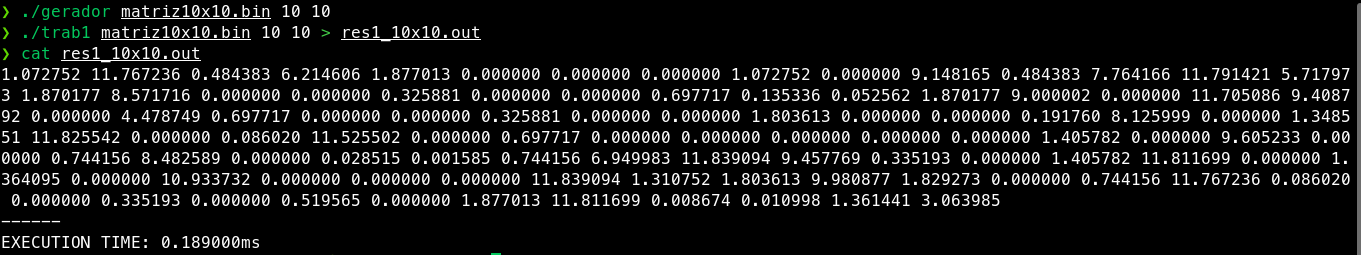
\includegraphics[width=.8\textwidth]{figuras/img1.png}
\end{figure}

\subsection{\esp Teste em matrizes maiores}
Para essa etapa, um programa alterado foi feito: "media\_trab1.c". A única diferença dele para o original é que ele recebe dois limites a e b na chamada e gera  5 matrizes de tamanhos incrementais, de a x a até b x b, aumentando de 10 em 10 (ex.: 10x10 , 20x20, 30x30, ... , b x b), e retorna o tempo de execução médio para cada tamanho. Esse programa foi utilizado para encontrar o tempo de execução para matrizes de 10x10 até 1000x1000 elementos (resultados salvos no arquivo "res\_media\_original.out") - a seguir encontra-se um gráfico com os resultados obtidos (curva azul), além de uma função de tempo aproximada calculada com regressão polinomial (curva vermelha) e o quoeficiente R² (que representa o quão próxima a função é dos valores verdadeiros):


% Figura
\begin{figure}[!ht]
	\centering	
	\caption[\hspace{0.1cm}Tempo de execução médio do programa original]{Tempo de execução médio do programa original}
	  \vspace{-0.4cm}
	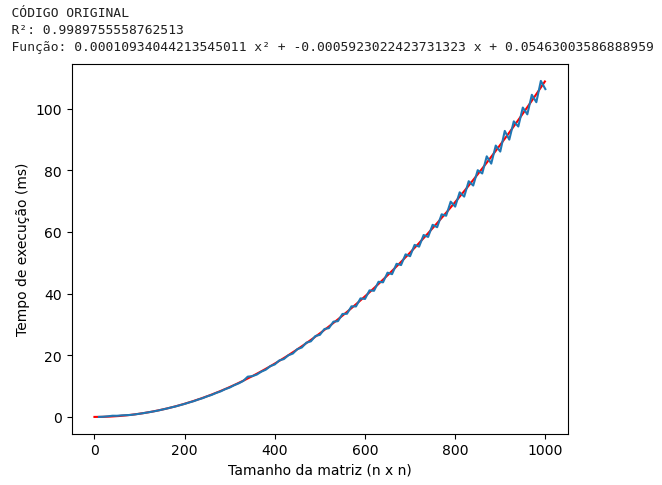
\includegraphics[width=.8\textwidth]{figuras/original.png}
\end{figure}

\newpage
\subsection{\esp Complexidade}
Observando o código, podemos chegar em uma função aproximada de custo f(n, m) = 13*n*m + 512 , para uma matriz de n linhas e m colunas. Com isso, podemos concluir que a complexidade do programa é O(n*m).



\section{\esp Melhorias}
\subsection{\esp Melhoria 1}
O programa original gera, para cada elemento da matriz, dois valores diferentes, "out\_even" (para elementos pares) e "out\_odd" (para elementos ímpares), e depois checa se o elemento é par ou ímpar e salva o que foi calculado em um array. Essa melhoria consiste em, ao invés de calcular tanto "out\_even" quanto "out\_odd" e depois salvar o valor, checar anteriormente se o número é par ou ímpar e fazer apenas um cálculo. O arquivo com o programa que implementa essa melhoria é o "melhoria1.c". 

\subsubsection{\esp Tempo de Execução Médio}
A seguir encontra-se o gráfico do tempo de execução médio do programa para matrizes de tamanhos diferentes: 

% Figura
\begin{figure}[!ht]
	\centering	
	\caption[\hspace{0.1cm}Tempo de execução médio - melhoria 1]{Tempo de execução médio - melhoria 1}
	  \vspace{-0.4cm}
	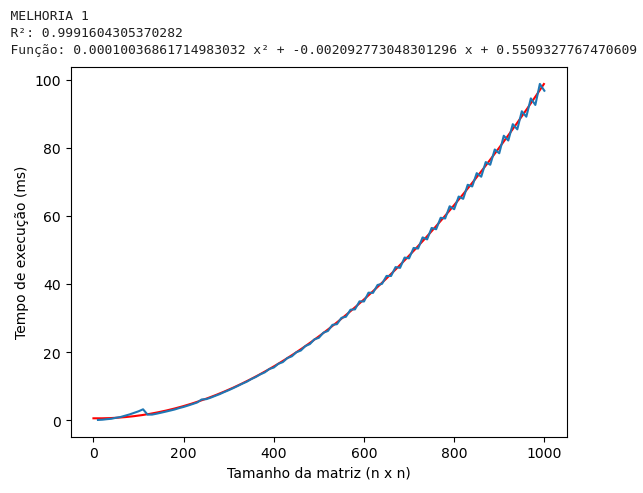
\includegraphics[width=.8\textwidth]{figuras/melhoria1.png}
\end{figure}

\subsubsection{\esp Speedup}

O seguinte gráfico representa o speedup do programa melhorado em relação ao programa original, para tamanhos de matrizes diferentes.

% Figura
\begin{figure}[!ht]
	\centering	
	\caption[\hspace{0.1cm}Speedup da melhoria 1]{Speedup da melhoria 1}
	  \vspace{-0.4cm}
	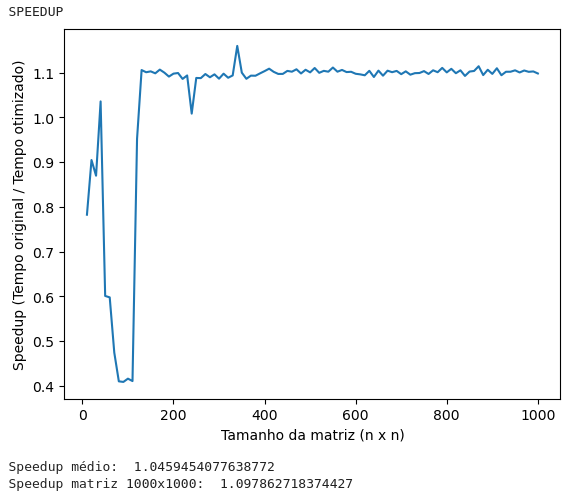
\includegraphics[width=.8\textwidth]{figuras/speedup_melhoria1.png}
\end{figure}

O speedup médio foi de aprox. 4,5945\%, e o speedup para uma matriz 1000x1000 de aprox. 9,7863\%. Podemos observar no gráfico que o comportamento para matrizes pequenas é pouco previsível, e que se torna mais estável ao aumentarmos o tamanho.

\subsection{\esp Melhoria 2}
Essa melhoria está relacionada ao array que conta a quantidade de cada elemento na matriz. Originalmente, se era feita a leitura da matriz em um loop, e depois um outro loop iterava sobre a matriz incrementando os contadores. A segunda melhoria consiste em incrementar os contadores após a leitura do elemento, evitando acessos repetidos à memória.

\subsubsection{\esp Tempo de Execução Médio}
A seguir encontra-se o gráfico do tempo de execução médio do programa para matrizes de tamanhos diferentes: 

% Figura
\begin{figure}[!ht]
	\centering	
	\caption[\hspace{0.1cm}Tempo de execução médio - melhoria 2]{Tempo de execução médio - melhoria 2}
	  \vspace{-0.4cm}
	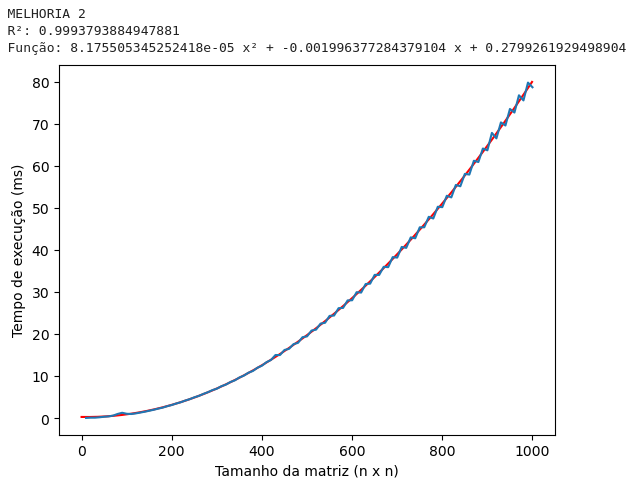
\includegraphics[width=.8\textwidth]{figuras/melhoria2.png}
\end{figure}

\subsubsection{\esp Speedup}
O seguinte gráfico representa o speedup do programa melhorado em relação ao programa original, para tamanhos de matrizes diferentes.

% Figura
\begin{figure}[!ht]
	\centering	
	\caption[\hspace{0.1cm}Speedup da melhoria 2]{Speedup da melhoria 2}
	  \vspace{-0.4cm}
	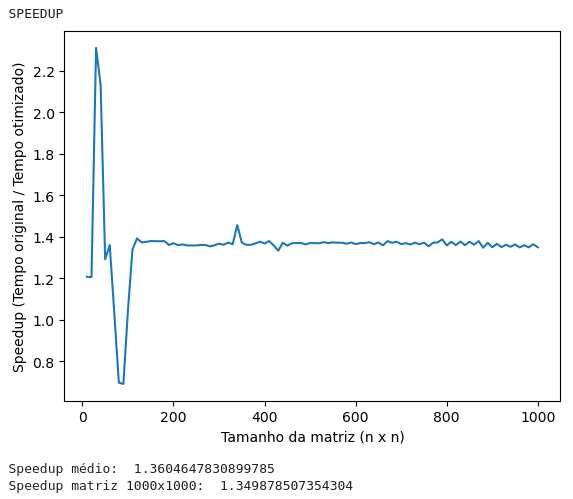
\includegraphics[width=.8\textwidth]{figuras/speedup_melhoria2.png}
\end{figure}

O speedup médio foi de aprox. 36,0465\%, e o speedup para uma matriz 1000x1000 de aprox. 34,9879\%. Houve um aumento de aprox. 31,4520\% do speedup médio ao adicionarmos a melhoria 2.

\subsection{\esp Melhoria 3}
A terceira melhoria implementa um array com os valores do seno e cosseno de 0 a 255º. A probabilidade de existirem dois elementos iguais em um conjunto de 58 números aleatórios entre 0 e 255 é maior que 99\% (aproximação obtida com a expansão da equação do Paradoxo do Aniversário utilizando a Série de Taylor) - portanto, para matrizes com mais de 58 elementos, podemos presumir que algum/alguns dos valores de seno e cosseno utilizados na função DetOutput provavelmente iriam ser calculados mais de uma vez. Essa melhoria apenas é aplicada, portanto, quando o número de elementos na matriz for maior que 58 (a função chamada é a DetOutputLargeMatrix nesse caso).

\newpage

\subsubsection{\esp Tempo de Execução Médio}
A seguir encontra-se o gráfico do tempo de execução médio do programa para matrizes de tamanhos diferentes: 

% Figura
\begin{figure}[!ht]
	\centering	
	\caption[\hspace{0.1cm}Tempo de execução médio - melhoria 3]{Tempo de execução médio - melhoria 3}
	  \vspace{-0.4cm}
	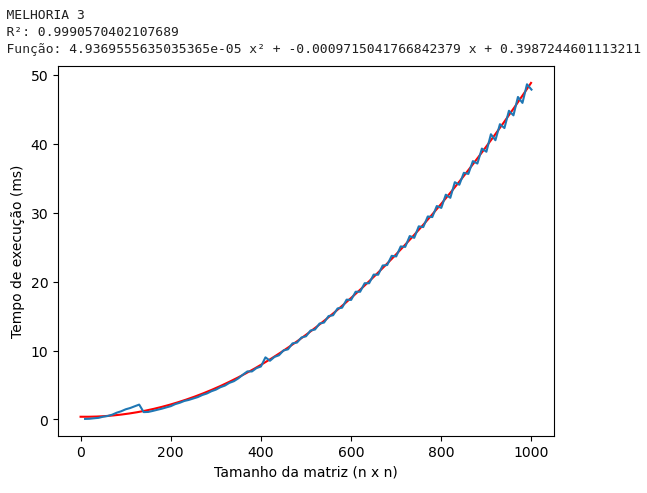
\includegraphics[width=.8\textwidth]{figuras/melhoria3.png}
\end{figure}

\subsubsection{\esp Speedup}
O seguinte gráfico representa o speedup do programa melhorado em relação ao programa original, para tamanhos de matrizes diferentes.

% Figura
\begin{figure}[!ht]
	\centering	
	\caption[\hspace{0.1cm}Speedup da melhoria 3]{Speedup da melhoria 3}
	  \vspace{-0.4cm}
	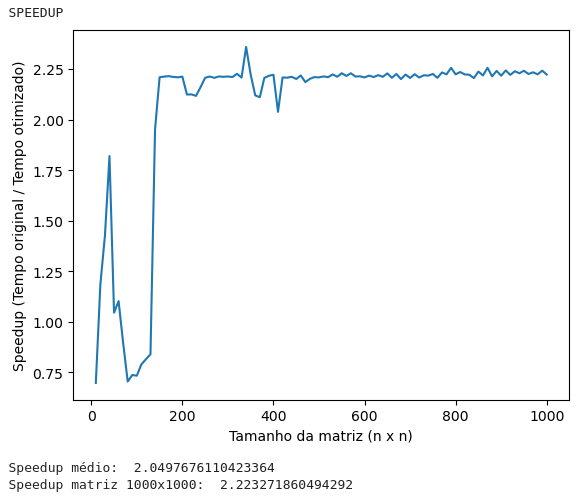
\includegraphics[width=.8\textwidth]{figuras/speedup_melhoria3.png}
\end{figure}

O speedup médio foi de aprox. 104,9768\%, e o speedup para uma matriz 1000x1000 de aprox. 122,3272\%. Houve um aumento de aprox 69,9303\% do speedup médio ao adicionarmos a melhoria 3. Essa melhoria é uma solução de compromisso, já que é necessário armazenar os valores calculados em memória - porém a quantidade de memória é ínfima comparada ao que o programa já gasta, e o grande speedup implica um ótimo custo/benefício.

\newpage

\subsection{\esp Melhoria 4}
A quarta melhoria consiste na mudança de uma operação aritmética para uma lógica (operações lógicas são executadas com muito mais facilidade no processador). Ao invés de utilizarmos a operação de módulo para ver se um elemento é par ou ímpar (funções DetOutput e DetOutputLargeMatrix), podemos realizar um "and" (&) entre o elemento e o número 1 - essa operação cria uma "máscara" que retorna apenas o bit menos significante do elemento, se esse bit for 0 o elemento é par e, se ele for 1, ímpar. 

\subsubsection{\esp Tempo de Execução Médio}
A seguir encontra-se o gráfico do tempo de execução médio do programa para matrizes de tamanhos diferentes: 

% Figura
\begin{figure}[!ht]
	\centering	
	\caption[\hspace{0.1cm}Tempo de execução médio - melhoria 4]{Tempo de execução médio - melhoria 4}
	  \vspace{-0.4cm}
	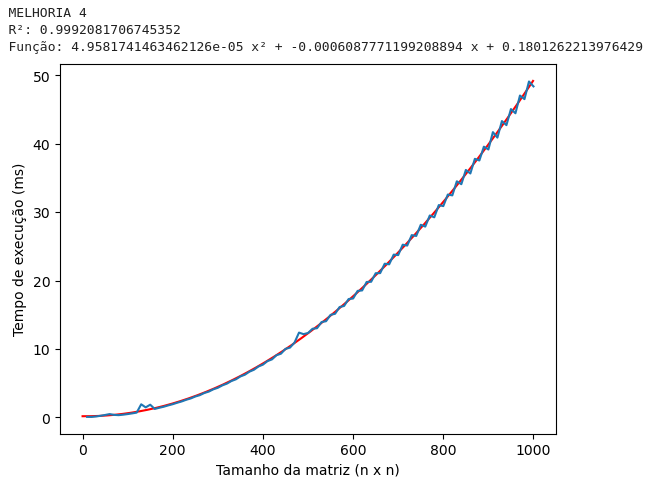
\includegraphics[width=.8\textwidth]{figuras/melhoria4.png}
\end{figure}

\newpage

\subsubsection{\esp Speedup}
O seguinte gráfico representa o speedup do programa melhorado em relação ao programa original, para tamanhos de matrizes diferentes.

% Figura
\begin{figure}[!ht]
	\centering	
	\caption[\hspace{0.1cm}Speedup da melhoria 4]{Speedup da melhoria 4}
	  \vspace{-0.4cm}
	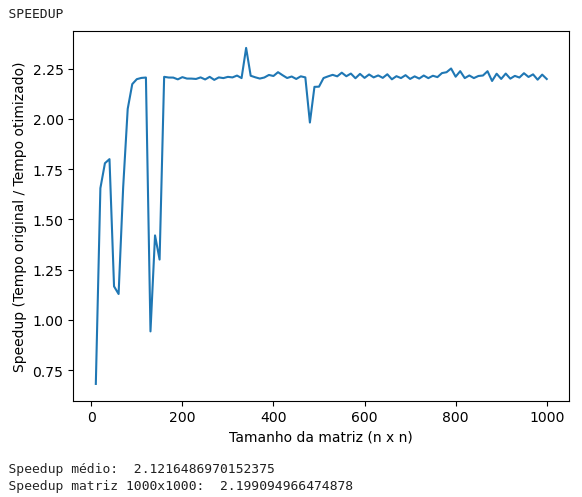
\includegraphics[width=.8\textwidth]{figuras/speedup_melhoria4.png}
\end{figure}

O speedup médio foi de aprox. 112,1649\%, e o speedup para uma matriz 1000x1000 de aprox. 119,9095\%.  Houve um aumento de aprox 7,1881\% do speedup médio ao adicionarmos a melhoria 4. 

\subsection{\esp Melhoria 5 (Final)}
Uma operação é executada sobre o array de contadores: caso a quantidade de um elemento seja maior que 0, o valor no array de contadores é alterado para o logaritmo da quantidade. Originalmente, essa operação é feita sobre todos os elementos do array - entretanto, o valor presente no array apenas é utilizado quando estamos determinando o output de um elemento ímpar. Dessa forma, podemos calcular o logaritmo apenas para as posições ímpares do array. 

\subsubsection{\esp Tempo de Execução Médio}
A seguir encontra-se o gráfico do tempo de execução médio do programa para matrizes de tamanhos diferentes: 

% Figura
\begin{figure}[!ht]
	\centering	
	\caption[\hspace{0.1cm}Tempo de execução médio - código final]{Tempo de execução médio - código final}
	  \vspace{-0.4cm}
	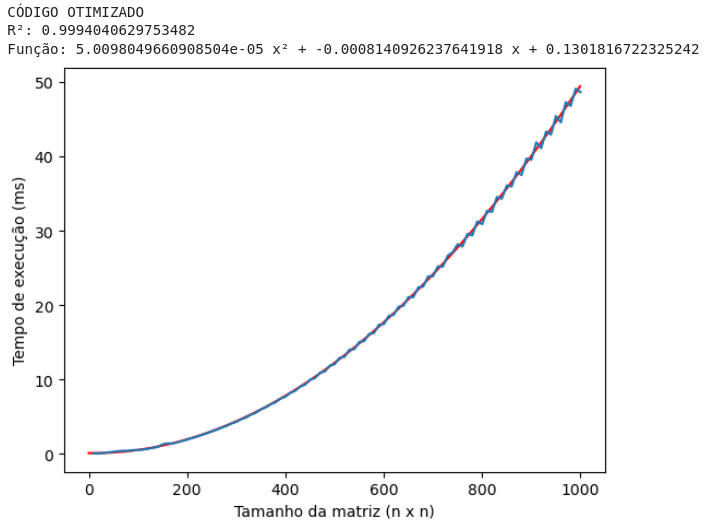
\includegraphics[width=.8\textwidth]{figuras/otimizado.png}
\end{figure}

\subsubsection{\esp Speedup}
O seguinte gráfico representa o speedup do programa melhorado em relação ao programa original, para tamanhos de matrizes diferentes.

% Figura
\begin{figure}[!ht]
	\centering	
	\caption[\hspace{0.1cm}Speedup do código final]{Speedup do código final}
	  \vspace{-0.4cm}
	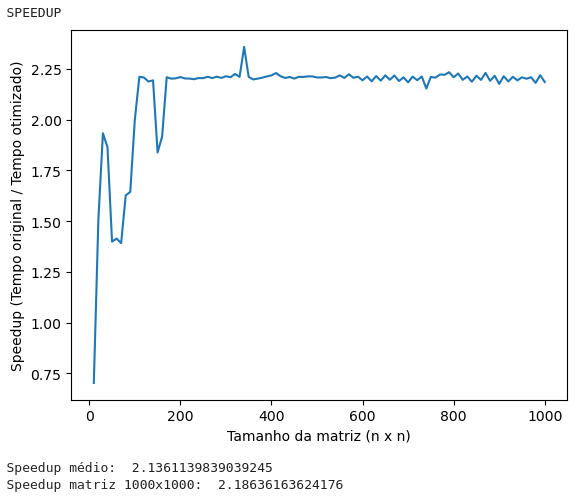
\includegraphics[width=.8\textwidth]{figuras/speedup_otimizado.png}
\end{figure}

O speedup médio foi de aprox. 113,6114\%, e o speedup para uma matriz 1000x1000 de aprox. 118,6362\%.  Houve um aumento de aprox 1,4465\% do speedup médio ao adicionarmos a melhoria 5. 


\newpage

\section{\esp CONCLUSÃO}
O código otimizado com as 5 melhorias apresentou tempos de execução mais que 2 vezes melhores que do original. Apesar disso, a complexidade permaneceu a mesma: para matrizes com menos de 59 elementos, as funções de custo para o melhor, o médio e o pior caso são, respectivamente, \(f1(n, m) = 7*n*m + 384\), \(f2(n, m) = 7,5*n*m + 384\), \(f3(n, m) = 8*n*m + 384\); já para matrizes com mais de 59 elementos, \(f1(n, m) = 6*n*m + 1152\), \(f2(n, m) = 6,5*n*m + 1152\), \(f3(n, m) = 7*n*m + 1152\). O pior caso é quando todos os elementos forem pares, e o melhor quando todos forem ímpares.
A seguir encontra-se a tela monstrando que o output do código otimizado e do código original foram iguais:

% Figura
\begin{figure}[!ht]
	\centering	
	  \vspace{-0.4cm}
	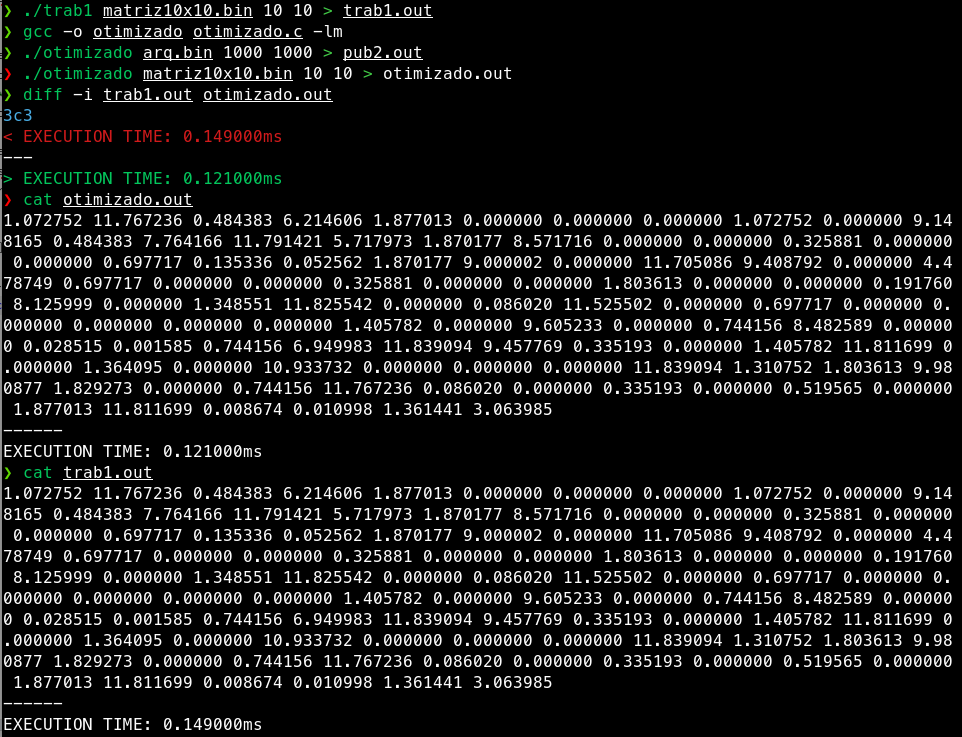
\includegraphics[width=1\textwidth]{figuras/diferenca_output.png}
\end{figure}

